\documentclass[12pt]{article}
\usepackage[utf8]{inputenc}
\usepackage{graphicx}
\usepackage{natbib}

\title{Computer Architecture Final Report}
\author{Walter Hill}
\date{December 6, 2019}

\begin{document}

\maketitle

\section{Background}


\subsection{Project Statement}\label{What}
\noindent This project will focus on re-implementing my own vector C++ functions using MASM assembly and then linking the assembly implementations with my existing C++ vector math library.  The math library was built for use within my in-development 3d graphics engine. The functions to be implemented in assembly are getMagnitude(), and cross(), performing a magnitude of a vector calculation and the cross product calculation respectively. The functions will be implemented with a focus on effective translation and efficiency.

\subsection{Goals}\label{Why}
\noindent The first goal is to become more proficient at translating high level code into assembly and vice versa. Through that process I hope to gain a better understanding of low level code optimization The other goal will be to attempt to make the Vector class functions run more efficiently both in isolation and ultimately within its use as a supplemental library. Lastly, it is my hope that undertaking this project will give me an increased understanding of vector and vector math as well. 

\subsection{Methods}\label{How}
\noindent This project will be achieved with the use of a number of development tools. Visual Studio will be the IDE of choice for this project, while version control will be handled using Git. A Visual Studio project currently exists for the vector math library. The assembly code with be written in MASM. The goal is for all MASM assembly code will be written within that project space, for the purposes of easy comparison, benchmarking, and eventual integration with the larger library. 

\subsection{Potential Challenges}\label{Potential Challenges}
\noindent Looking ahead, I envision the obstacles that occur in this project will come from the process of translating from C++ to assembly primarily. Porting the implementation one to one might turn out to be a manageable task, but I think further challenge will come as a result of attempting to write the given C++ functions more efficiently in MASM. I believe that will require full use of the assembly knowledge I have gained over the course of this semester. Setting up the benchmarking environment will take significant care as well. It will be important to make sure the efficiency tests are run in a way that accurately showcases the strengths and weaknesses of both the assembly and C++ implementations. 

\section{Implementation}
\subsection{Test Details}
The test project was built using Visual Studio and Visual Studio's C++ and MASM compilers on the x86 architecture. Control flow was initialized within the main.cpp file. All MASM functions were defined as extern and utilized the C calling convention. All MASM functions declared in the C++ file began with an underscore to denote their assembly implementation. The test began by testing the MASM implementation of the Vector3 cross() and Vector3 getMagnitude() functions. The result of the function calls were displayed to the console window. 
\newline
\newline

\begin{figure}[!htb]
  \centering
  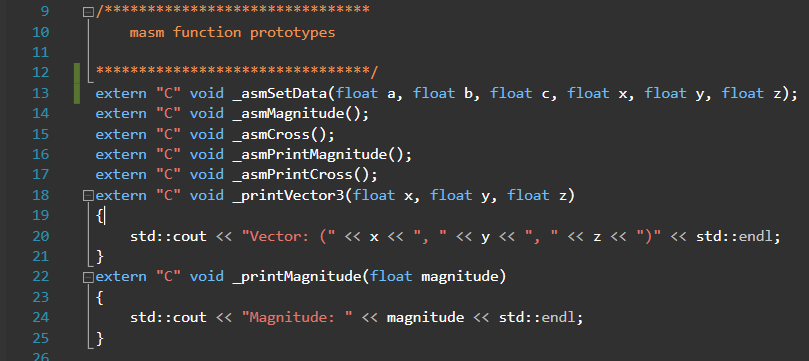
\includegraphics[scale=0.7]{img/masm_func.PNG}
  \caption{MASM function declarations}
  \label{fig:masm_func}
\end{figure}

\noindent Second, the benchmark test was run as a function defined as runAsmCppBenchmark(). This test compared the MASM implementation of cross() to the C++ implementation of the function created within the Vector3 class as well as the MASM implementation of getMagnitude() to its own C++ counterpart. The comparison itself was benchmarked using a high frequency timer reporting its timing in milliseconds. The timer was implemented as a separate class called RK\_Timer, and the class utilized the C++ chrono library for time tracking and reporting. 

For this report, each MASM and C++ function was called 1 million times based on the value of a constant variable named NUM\_TEST\_RUNS. For each loop iteration in which the Vector3 functions were called, the Vector3 data utilized for the calculations was randomized. This randomization was performed using the C++ random library and a random\_device object to ensure effective randomization for both cross() and getMagnitude() respectively. The time reported for each iteration of the for loop was then stored in a std::vector of doubles. After the loop concluded, in the case of the cross() test and the getMaginutude() test, the std::vector of time values was averaged out into a single average time in milliseconds and reported out to the console.

\begin{figure}[!htb]
  \centering
  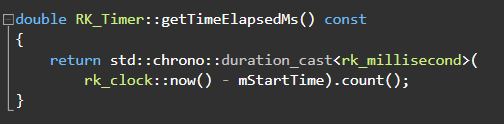
\includegraphics[scale=0.75]{img/time_func.PNG}
  \caption{RK\_Timer definition returns time since start in milliseconds.}
  \label{fig:time_func}
\end{figure}

\subsection{MASM Details}
The MASM code implementation made extensive use of the ST registers and the x87 floating point architecture including in cross() and getMagnitude(). Vector data was stored as three individual REAL4 floating point values declared in the DATA segment. 

The cross() and getMagnitude() functions both made heavy use of the fld and fmul commands to store data in the FPU stack registers and multiply floating point values respectively. 

The MASM implementation also included functions whose sole purpose was to print out the results of cross() and getMagnitude() to test for effective translation and implementation of the Vector3 class functions.

\subsection{C++ Details}
The C++ implementation of cross() and getMagnitude are declared in the Vector3.h header file and implemented in Vector3.cpp. The cross() function differs from getMagnitude() as the cross function is declared as static. The cross function also differs slightly from its MASM counterpart due to the fact that the C++ implementation returns a Vector3 object comprised of the calculated float values, while the MASM version only stores the floating point numbers individually.

The Vector3 object is made up of three float variables that can be accessed through inline constant accessors. The function getX() for example returns the floating point member variable x.

\clearpage
\section{Solutions}
Reviewing the challenges, anticipated at the outset of this project, I believe I was able to meet and overcome those challenges. Translating the Vector3 functions from C++ to MASM took time, but did not turn out to be too heavy of a task. I was able to overcome that hurdle with the help of MASM floating point documentation references \cite{masm_fpu_docs}. 
\newline
\newline
Setting up the Visual Studio environment required adding a MASM compiler command to the Pre-Link Event field of the Visual Studio project. Without it, the project would fail to create an object file from the written MASM code. Setting up the IDE also required a subsystem change in the project files to define the subsystem for the project as Console (/SUBSYSTEM:CONSOLE). I found that without this subsystem definition, the project would fail to compile. For the solutions to the IDE setup, I was able to reference my previous Visual Studio projects to get this project up to speed quickly and with minimal confusion. 
\newline


\begin{figure}[!htb]
  \centering
  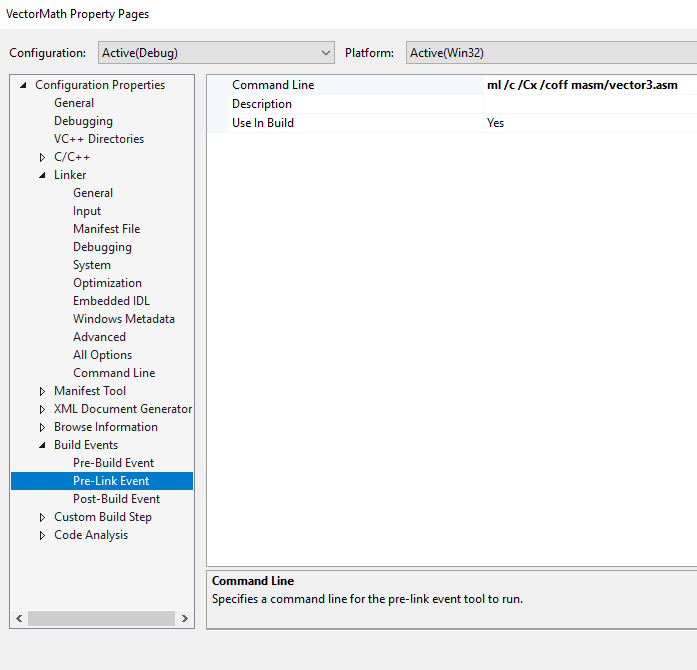
\includegraphics[scale=0.75]{img/link_event.PNG}
  \caption{MASM pre-linking compilation command.}
  \label{fig:link}
\end{figure}

\noindent Ensuring the benchmark test was set up in an objective and effective fashion required a lot of forethought when it came to the architecture of the project on both the C++ and assembly side. I attempted to account for all the areas where poorly structured code could negatively affect the data gathered. Despite this, I discovered, through debugging, that test results were skewed in favor of the C++ getMagnitude() function due to compiler optimizations. I had been utilizing the same Vector3 variable for each iteration of the function call. This meant that on the C++ side, the compiler was performing unspoken optimizations that resulted in the C++ functions taking longer than MASM functions initially, then dropping off to a much faster execution rate on subsequent calls. To fix this, I randomized the Vector3 variables for each call, to eliminate the possibility of compiler optimization on the data used during testing. This meant that the randomized variables had to be passed to the assembly functions as well. To accomplish this, I added an additional extern assembly function to store the randomized variable data in assembly variables declared in the DATA segment. This change resulted in much more accurate benchmark data and a more effective test overall. 
\newline
\newline
Ultimately, the challenge of implementing more efficient MASM functions was met with mixed success. For further detail on function speed, see the results section below. Overall, the challenges encountered on this project proved solvable and were overcome with the help of documentation, previous work, and debugging the project code with a close eye.

\clearpage
\section{Results}
The first round of testing was done in Visual Studio's Debug mode without the debugger active. The second set of tests were performed in Visual Studio and set to Release mode without the debugger active.

\begin{figure}[!htb]
  \centering
  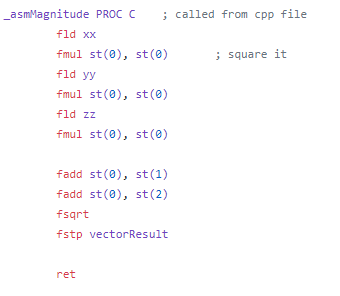
\includegraphics[scale=1]{img/asmMagnitude.PNG}
  \caption{MASM getMagnitude() implmentation. }
  \label{fig:asmmag}
\end{figure}

\subsection{getMagnitude() - Debug Mode}
When observing the results for getMagnitude after 1 million function calls, it is apparent that the MASM version of getMagnitude() is about 0.00003 milliseconds faster than its C++ counterpart. While this difference is marginal in a real world scenario, the following paragraph will attempt to understand why this result occurred. 

Upon review of the assembly code in comparison to the c++ code, one possible reason for the given result could be the increased efficiency of the floating point square root function (fsqrt) in MASM when compared to C++'s sqrtf() function. Another cause of this result could be attributed to the speed of MASM's direct access to the FPU registers. The getMagnitude() function operates by first squaring the three float variables of the Vector3 object, adding the three products, and then square roots the sum. 

The MASM version of getMagnitude() performs its squaring multiplication (using fmul) simply by multiplying the ST0 floating point register by itself. The C++ version of getMagnitude performs its squaring multiplication by squaring the three float member variables of the Vector3 class. It is possible that the edge in speed that the MASM implementation holds comes as a result of the C++ version of getMagnitude() making marginally less effective use of floating point registers. This conclusion could be reached given that squaring two non-register variables would also include two register loading operations from dynamic into static memory for each of member variable reference before calculations could be performed. 

\begin{figure}[!htb]
  \centering
  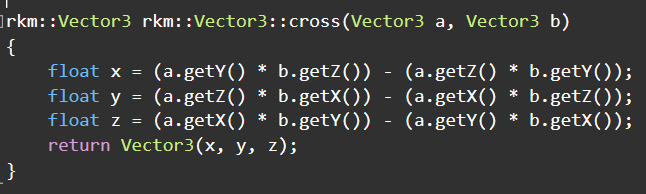
\includegraphics[scale=0.8]{img/cross.PNG}
  \caption{C++ cross product implementation.}
  \label{fig:cross}
\end{figure}

\subsection{cross() - Debug Mode}
When observing the results for the cross() function after 1 million calls, the results illustrate that the C++ version of the cross() function runs approximately 0.0001 milliseconds faster that the MASM implementation. When observing this time difference, it is clear that the C++ implementation has a clear, if impercetible, edge over the MASM version of the function. When inspecting the MASM function for answers, it would appear the function performs many more calls to dynamic memory to retrieve variable data for aritmetic operations on the FPU than its C++ counterpart. When in the realm of thousandths of milliseconds, these calls out to dynamic memory can take a non-insignificant amount of time. In the MASM implementation, variables are loaded into the FPU twelve times per function call which certainly contributes to the slower average run time.

\begin{figure}[!htb]
  \centering
  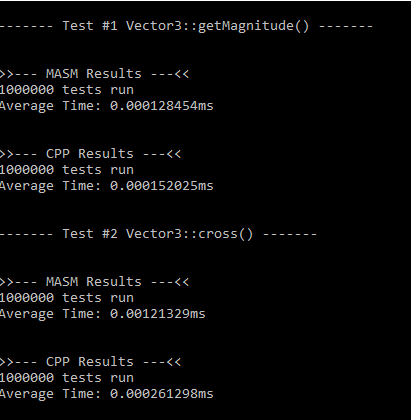
\includegraphics[scale=1.25]{img/debug_results.PNG}
  \caption{Benchmark report in x86 Debug mode.}
  \label{fig:debug}
\end{figure}


\subsection{getMagnitude() - Release Mode}
Reviewing the getMagnitude() test results in review mode presents much the same outcome as the Debug mode testing, albeit with greater optimizations performed on both the MASM and C++ implementations. 

The timing results between both implementations was even more tightly grouped in the Release mode with the MASM implementation running at \[8.5x10^-5ms\]
and the c++ implementation running at an average of \[8.9x10^-5ms\]
The MASM function is still the faster of the two, but the difference in Release mode is even more granular.

\subsection{cross() - Release Mode}
Observing the Release mode results for the cross() function presents data in line with the Debug mode findings. The MASM implementation continues to trail behind the C++ version. In Release mode, that gap is even wider thanks to the  increase in optimizations performed by the C++ compiler. 

The timing results between both implementations was spread even further in the Release mode with the MASM implementation running at a slower \[4.9x10^-3ms\] with the c++ implementation running at a speedy average of \[9.5x10^-5ms\]
The MASM cross() function remains the slower of the two, but the difference in Release mode is noticeably steeper especially at such a small scale, making it apparent that the inefficiency of the MASM cross() places on not insignificant burden on its performance.

\begin{figure}[!htb]
  \centering
  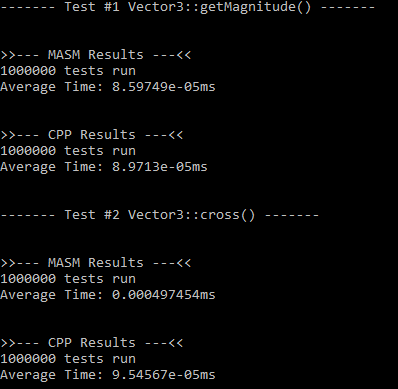
\includegraphics[scale=1.25]{img/release_results.PNG}
  \caption{Benchmark report in x86 Release mode.}
  \label{fig:relase}
\end{figure}

\clearpage
\bibliographystyle{plain}
\bibliography{references}

\end{document}
